\subsection{平面图形的面积}
\subsubsection{直角坐标情形}
\paragraph{}
应用定积分,可以计算一些比较复杂的平面图形的面积。

\paragraph{}
\textbf{例子1\;}计算抛物线$y^2=2x$与直线$y=x-4$所围成的图形的面积

\begin{figure}[H]
\centering
  % 直角坐标的定积分应用
\begin{tikzpicture}[scale=0.8]
  \begin{axis}[clip=false,xmin=0, xmax=10,ymin=-5,ymax=5, grid=none,
    xtick=\empty, ytick=\empty, axis lines=middle,
    smooth, xlabel={$x$}, ylabel={$y$}]

    % 曲线: y^2=2x,y=x-4
    \addplot[draw=red,domain=0:9,samples=150] {sqrt(2*x)};
    \addplot[draw=red,domain=0:9,samples=150] {-sqrt(2*x)};
    \addplot[draw=blue,domain=0:9] {x-4};

    \node [right] at (2.4,-1.8) {$(2,-2)$};
    \node [below right] at (7.8,4) {$(8,4)$};

    \node [above] at (9,5) {$y=x-4$};
    \node [above left] at (7,3.74) {$y^2=2x$};

    \node [left] at (0,2.7) {$y + dy$};
    \node [left] at (0,2) {$y$};

    \draw [dashed] (0,2.7) -- (6.7,2.7);
    \draw [dashed] (0,2) -- (6,2);

    \draw [pattern=north east lines] (2,2) rectangle (6,2.7);


    \draw [dashed,draw=cyan] (0,-2) -- (9,-2);
    \draw [dashed,draw=cyan] (0,4) -- (9,4);

    % 原点
    \node [below left] at (0,0) {$O$};
  \end{axis}
\end{tikzpicture}

  \caption{抛物线与直线围成的面积}
\end{figure}

\paragraph{}
\textbf{解\;}为了确定图形的区间,先求出抛物线和直线的交点,解方程组
\begin{equation*}
  \left\{ \begin{array}{l}
    y^2 \;=\; 2x, \\
    y \;=\; x - 4,
  \end{array} \right.
\end{equation*}
得交点$(2,-2)$和$(8,4)$,从而知道这图形在直线$y=-2$及$y=4$之间。

\paragraph{}
现在,选取纵坐标$y$为积分变量,它的变化区间为$[-2,4]$(选取横坐标$x$为积分变量不方便)。

\paragraph{}
$[-2,4]$上任一小区间$[y,y+dy]$的窄条面积近似于高为$dy$、底为$\displaystyle(y+4)-\frac{1}{2}y^2$的窄矩形的面积,从而得到面积元素
\begin{equation*}
  dA = \big( y+4-\frac{1}{2}y^2 \big)dy.
\end{equation*}
以$\displaystyle\big( y+4-\frac{1}{2}y^2 \big)dy$为被积表达式,在闭区间$[-2,4]$上作定积分,便得所求的面积为
\begin{align*}
  A \;=&\; \int_{-2}^4\big( y+4-\frac{1}{2}y^2 \big)dy \\
  =&\; \big[ \frac{y^2}{2} + 4y - \frac{y^3}{6} \big]_{-2}^4 \\
  =&\; 18.
\end{align*}

\subsubsection{极坐标情形}
\paragraph{}

设由曲线$\rho=\varphi(\theta)$及射线$\theta=\alpha, \theta=\beta$围成一图形,现在要计算它的面积。这里,$\varphi(\theta)$在$[\alpha,\beta]$上连续,且$\varphi(\theta) \geq 0$。

\begin{figure}[H]
\centering
  % 极坐标的定积分应用
\begin{tikzpicture}[scale=1.5]
  \begin{polaraxis}[
    clip=false,ticks=none,grid=none,ylabel={$x$},
    axis lines=middle,x axis line style = {transparent},
    xmin=0,xmax=40,ymin=0,ymax=170,font=\tiny
  ]

    % ρ = φ(θ)
    \addplot[red,domain=10:40,samples=100] (x, {150+x/2)});
    \node [red,below right] at (40,175) {$\rho=\varphi(\theta)$};

    % alpha
    \addplot[blue,domain=0:155] (10, x);
    \addplot[blue,domain=0:10] (x,50);
    \node [blue] at (5,55) {$\alpha$};

    % beta
    \addplot[cyan,domain=0:170] (40, x);
    \addplot[cyan,domain=0:40] (x, 70);
    \node [cyan,rotate=15] at (15,75) {$\beta$};

    % θ
    \addplot[domain=0:20] (x, 90);
    \node [rotate=5] at (5,95) {$\theta$};

    % θ + dθ
    \addplot[domain=0:30] (x, 110);
    \node [right,rotate=5] at (5,107) {$\theta + d\theta$};

    \filldraw[pattern=north east lines] (0,0) -- (20,160) arc (20:30:32mm) -- cycle;

    % dθ
    \addplot[domain=20:30] (x, 130);
    \node [fill=white,right,rotate=25, inner sep = 1] at (25,130) {$d\theta$};

    % 原点
    \node [below left] at (0,0) {$O$};
  \end{polaraxis}
\end{tikzpicture}

  \caption{曲边扇形}
\end{figure}

\paragraph{}
由于当$\theta$在$[\alpha,\beta]$上变动时,极径$\rho=\varphi(\theta)$也随之变动,因此所求图形的面积不能直接利用扇形面积的公式$\displaystyle A=\frac{1}{2}R^2\theta$来计算。

\paragraph{}
取极角$\theta$为积分变量,它的变化区间为$[\alpha,\beta]$。相应于任一小区间$[\theta, \theta+d\theta]$的窄曲边扇形的面积可以用半径为$\rho=\varphi(\theta)$、中心角为$d\theta$的扇形的面积来近似代替,从而得到这窄曲边扇形面积的近似值,即曲边扇形的面积元素

\begin{equation*}
  dA = \frac{1}{2}[\varphi(\theta)]^2d\theta.
\end{equation*}

以$\displaystyle\frac{1}{2}[\varphi(\theta)]^2d\theta$为被积表达式,在闭区间$[\alpha,\beta]$上作定积分,便得所求曲边扇形的面积为
\begin{equation*}
  A = \int_\alpha^\beta\frac{1}{2}[\varphi(\theta)]^2d\theta.
\end{equation*}

\subsection{体积}
\subsubsection{旋转体的体积}
\paragraph{}
\uwave{旋转体}就是由一个平面图形绕这平面内一条直线,旋转一周而成的立体,这直线叫做\uwave{旋转轴}。

\begin{figure}[H]
\centering
  % 旋转体的体积, solid of revolution
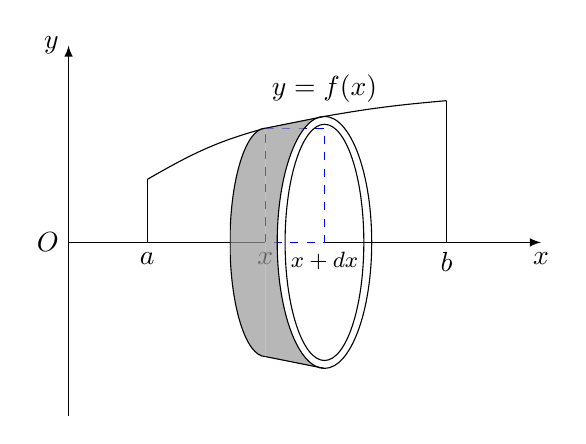
\begin{tikzpicture}[scale=1]
  % \draw [help lines] (-3,-3) grid (3,3);

  % 坐标
  \node[left] at (0,2.5) {$y$};
  \draw[-latex] (0,-2.2) -- (0,2.5);
  \node[below] at (6,0) {$x$};
  \draw (0,0) -- (2.5,0);
  \draw[-latex] (3.25,0) -- (6,0);
  \node[left] at (0,0) {$O$};

  % y=f(x)
  \node[above] at (3.25,1.65) {$y=f(x)$};
  \draw (1,0.8) to [out=30,in=195] (2.5,1.45);
  \draw (3.25,1.6) to [out=10,in=185] (4.8,1.8);

  % 端点
  \node[below] at (1,0) {$a$};
  \draw (1,0.8) -- (1,0);
  \node[below] at (4.8,0) {$b$};
  \draw (4.8,1.8) -- (4.8,0);

  \node[below] at (2.5,0) {$x$};
  \node[below] at (3.25,0) {\footnotesize $x + dx$};
  \draw[dashed, blue] (2.5,1.45) -- (3.25,1.45) -- (3.25,0) -- (2.5,0) -- (2.5,1.45);

  % ----------------------------------------------------------------------------

  % 左边椭圆和填充
  \begin{scope}
    \pgfsetfillopacity{0.7}
    \clip (2.05,-1.47) rectangle (2.501,1.47);
    \draw[fill=black!40] (2.5,0) ellipse [x radius=0.45cm,y radius=1.45cm];
  \end{scope}
  % 填充
  \begin{scope}
    \clip (2.4,-1.6) rectangle (3.24,1.6); % 3.25 --> 3.24,移除精度导致的黑线
    \pgfsetfillopacity{0.7}
    \path[fill=black!40,even odd rule] (2.5,1.45) -- (3.25,1.6) -- (3.25,-1.6) -- (2.5,-1.45) -- (2.5,1.45)
    (3.25,0) ellipse [x radius=0.6cm,y radius=1.6cm];
  \end{scope}

  % 右边椭圆
  \draw (3.25,0) ellipse [x radius=0.6cm,y radius=1.6cm];
  \draw (3.25,0) ellipse [x radius=0.5cm,y radius=1.5cm];

  % 椭圆上下边线
  \draw (2.5,1.45) -- (3.25,1.6);
  \draw (2.5,-1.45) -- (3.25,-1.6);
\end{tikzpicture}

  \caption{旋转体体积}
  \label{旋转体体积}
\end{figure}

\paragraph{}
上述旋转体都可以看作是由连续曲线$y=f(x)$、直线$x=a$、$x=b$及$x$轴所围成的曲边梯形绕$x$轴旋转一周而成的立体。现在下面用定积分来计算这种旋转体的体积。

\paragraph{}
取横坐标$x$为积分变量,它的变化区间为$[a,b]$。相应于$[a,b]$上的任一小区间$[x,x+dx]$的窄曲边梯形绕$x$轴旋转而成的薄片的体积近似于以$f(x)$为底半径、$dx$为高的扁圆柱体的体积(图 \figureref{旋转体体积}),即体积元素

\begin{equation}
  dV = \pi[f(x)]^2dx.
\end{equation}

\paragraph{}
以$\pi[f(x)]^2dx$为被积表达式,在闭区间$[a,b]$上作定积分,便得所求旋转体体积为

\begin{equation}
  V = \int_a^b\pi[f(x)]^2dx.
\end{equation}

\subsubsection{平行截面面积为已知的立体的体积}
\paragraph{}
从计算旋转体体积的过程中可以看出:如果一个立体不是旋转体,但却知道该立体上垂直于一定轴的各个截面的面积,那么,这个立体的体积也可以用定积分来计算。

\begin{figure}[H]
\centering
  % 已知平行截面面积的立体的体积
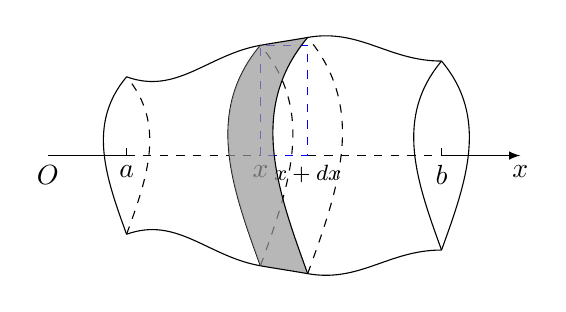
\begin{tikzpicture}[scale=1]
  % \draw [help lines] (0,-3) grid (6,3);

  \draw (0,0) -- (1,0);
  \draw[dashed] (1,0) -- (2.7,0);
  \draw[dashed] (3.3,0) -- (5,0);
  \draw[-latex] (5,0) -- (6,0);
  \node[below] at (0,0) {$O$};
  \node[below] at (1,0) {$a$};
  \draw (1,0) -- (1,0.1);
  \node[below] at (6,0) {$x$};
  \node[below] at (5,0) {$b$};
  \draw (5,0) -- (5,0.1);
  \node[below] at (2.7,0) {$x$};
  \node[below] at (3.3,0) {\footnotesize $x+dx$};
  \draw[dashed,blue] (2.7,0) -- (2.7,1.4) -- (3.3,1.4) -- (3.3,0) -- (2.7,0);

  % 左边
  \draw (1,-1) to [out=110,in=230] (1,1);
  \draw[dashed] (1,-1) to [out=70,in=-50] (1,1);

  % 左边的边框
  \draw (1,1) to [out=-20,in=190] (2.7,1.4);
  \draw (1,-1) to [out=20,in=170] (2.7,-1.4);

  % 中间 1
  \draw (2.7,-1.4) to [out=110,in=230] (2.7,1.4);
  \draw[dashed] (2.7,-1.4) to [out=70,in=-50] (2.7,1.4);

  % 阴影
  \begin{scope}
    \pgfsetfillopacity{0.7}
    \path[fill=black!40] (2.7,-1.4) to [out=110,in=230] (2.7,1.4) to [out=10,in=190] (3.3,1.5) to [out=230,in=110] (3.3,-1.5) to [out=170,in=-10] (2.7,-1.4);
  \end{scope}

  % 中间的边框
  \draw (2.7,1.4) to [out=10,in=190] (3.3,1.5);
  \draw (2.7,-1.4) to [out=-10,in=170] (3.3,-1.5);

  % 中间 2
  \draw (3.3,-1.5) to [out=110,in=230] (3.3,1.5);
  \draw[dashed] (3.3,-1.5) to [out=70,in=-50] (3.3,1.5);

  % 右边的边框
  \draw (3.3,1.5) to [out=10,in=180] (5,1.2);
  \draw (3.3,-1.5) to [out=-10,in=180] (5,-1.2);

  % 右边
  \draw (5,-1.2) to [out=110,in=230] (5,1.2);
  \draw (5,-1.2) to [out=70,in=-50] (5,1.2);
\end{tikzpicture}

  \caption{已知平行截面面积的立体的体积}
  \label{已知平行截面面积的立体的体积}
\end{figure}

\paragraph{}
如图\figureref{已知平行截面面积的立体的体积}所示,取上述定轴为$x$轴,并设该立体在过点$x=a$、$x=b$且垂直于$x$轴的两个平面之间。以$A(x)$表示过点$x$且垂直于$x$轴的截面面积。假定$A(x)$为$x$的已知的连续函数。这时,取$x$为积分变量,它的变化区间为$[a,b]$;立体中相应于$[a,b]$上任一小区间$[x,x+dx]$的一薄片的体积,近似于底面积为$A(x)$、高为$dx$的扁柱体的体积,即体积元素:
\begin{equation}
  dV = A(x)dx.
\end{equation}
以$A(x)dx$为被积表达式,在闭区间$[a,b]$上作定积分,便得所求立体的体积
\begin{equation}
  V = \int_a^bA(x)dx.
\end{equation}

\subsubsection{平面曲线的弧长}
\paragraph{}
圆的周长可以利用圆的内接正多边形的周长当边数无限增多时的极限来确定。现在用类似的方法来建立平面的连续曲线弧长的概念,从而应用定积分来计算弧长。

\begin{figure}[H]
\centering
  % 平面曲线的弧长
\begin{tikzpicture}[scale=0.8]
  \begin{axis}[clip=false,xmin=0, xmax=9,ymin=0,ymax=9, grid=none,
    xtick=\empty, ytick=\empty, axis lines=middle,
    smooth, xlabel={$x$}, ylabel={$y$}]

    % 曲线
    \addplot[domain=1.8:8] {-x^2/20 + x/6 + 1.5*ln(x - 1) + 4};

    \draw (1.8,3.8) -- (2.8,4.956) -- (3.8,5.46) -- (4.8,5.65) -- (5.8,5.64) -- (7.4,5.28) -- (8,5.05);
    \node[below] at (1.8,3.8) {$A=M_0$};
    \node[above left] at (2.8,4.956) {$M_1$};
    \node[above left] at (3.8,5.46) {$M_2$};

    \node[above] at (7.4,5.30) {$M_{n-1}$};
    \node[below] at (8,5.05) {$B=M_n$};

    % 原点
    \node [below left] at (0,0) {$O$};
  \end{axis}
\end{tikzpicture}

  \caption{平面曲线的弧长}
  \label{平面曲线的弧长}
\end{figure}

\paragraph{}
设$A, B$ 是曲线弧的两个端点。在弧$\overarc{AB}$上依次任取分点$A=M_0,M_1,M_2,\cdots,M_{i-1},M_i,\cdots$\\$,M_{n-1},M_n=B$,并依次连接相邻的分点得一折线(图\figureref{平面曲线的弧长})。当分点的数目无限增加且每个小段$\overarc{M_{i-1}M_i}$都缩向一点时,如果此折线的长$\displaystyle\sum_{i=1}^n|M_{i-1}M_i|$的极限存在,则称此极限为\uwave{曲线弧\text{$\overarc{AB}$}的弧长},并称此曲线弧$\overarc{AB}$是\uwave{可求长}的。

\paragraph{}
\textbf{定理\;}光滑曲线弧是可求长的。

\paragraph{}
下面利用定积分的元素法来讨论平面光滑曲线弧长的计算公式。

\paragraph{}
设曲线弧由参数方程

\begin{align}
\begin{split}
  \left\{\begin{array}{l} x=\varphi(t), \\ y = \psi(t) \end{array}\right. \; (\alpha \leq t \leq \beta)
\end{split}
\end{align}
给出,其中$\varphi(t), \psi(t)$在$[\alpha,\beta]$上具有连续导数,且$\varphi'(t), \psi'(t)$不同时为零。现在来计算这曲线弧的长度。

\paragraph{}
取参数$t$为积分变量,它的变化区间为$[\alpha,\beta]$。相应于$[\alpha,\beta]$上任一小区间$[t,t+dt]$的小弧段的长度$\Delta s$近似等于对应的弦的长度$\sqrt{(\Delta x)^2 + (\Delta y)^2}$。因为

\begin{align}
  \Delta x = \varphi(t+dt)-\varphi(t) \approx dx = \varphi'(t)dt, \\
  \Delta y = \psi(t+dt)-\psi(t) \approx dy = \psi'(t)dt,
\end{align}
所以,$\Delta s$的近似值(弧微分)即弧长元素为
\begin{align}
  ds \;=&\; \sqrt{(dx)^2 + (dy)^2} = \sqrt{\varphi'^2(t)(dt)^2 + \psi'^2(t)(dt)^2} \\
  \;=&\; \sqrt{\varphi'^2(t) + \psi'^2(t)}dt.
\end{align}
于是所求弧长为
\begin{equation}
  s = \int_\alpha^\beta\sqrt{\varphi'^2(t) + \psi'^2(t)}dt.
\end{equation}

\paragraph{}
当曲线弧由直角坐标方程
\begin{equation}
  y=f(x) \;\; (a \leq x \leq b)
\end{equation}
给出,其中$f(x)$在$[a,b]$上具有一阶连续导数,这时曲线弧有参数方程
\begin{align}
  \left\{\begin{array}{l}
    x = x, \\
    y = f(x)
  \end{array} \right. \; (a\leq x \leq b),
\end{align}
从而所求的弧长为

\begin{equation}
  s = \int_a^b\sqrt{1+y'^2}dx.
\end{equation}

\paragraph{}
当曲线弧由极坐标方程
\begin{equation}
  \rho = \rho(\theta) \;\; (\alpha \leq \theta \leq \beta)
\end{equation}
给出,其中$\rho(\theta)$在$[\alpha,\beta]$上具有连续导数,则由直角坐标与极坐标的关系可得
\begin{align}
  \left\{\begin{array}{ll}
    x \;= & \rho(\theta)\cos\theta, \\
    y \;= & \rho(\theta)\sin\theta
    \end{array}\right. \; (\alpha \leq \theta \leq \beta).
\end{align}
这就是以极角$\theta$为参数的曲线弧的参数方程。于是,弧长元素为
\begin{equation}
  ds = \sqrt{x'^2(\theta) + y'^2(\theta)}d\theta = \sqrt{\rho^2(\theta) + \rho'^2(\theta)}d\theta,
\end{equation}
从而所求弧长为
\begin{equation}
  s = \int_\alpha^\beta\sqrt{\rho^2(\theta) + \rho'^2(\theta)}d\theta.
\end{equation}
